\documentclass{report} 
\usepackage[thaifont = Angsana New]{thaispec} 
\usepackage{verbatim}
\usepackage{graphicx}
\title{ฐานข้อมูลบริษัทน้ำเปล่า} 
\author{
\begin{tabular}{ll}
นาย มนัฐยศ จิตรสมาน 116510901011-6\\
นางสาว อจิรวดี จันทวรรณ 116510901026-4\\
นาย ธรรศนนท์ แตงร่ม 116510901027-2\\
\end{tabular}\\ 
\\
เสนอ\\
ดร.รัฐพรหม พรหมคำ\\
\\
สาขาวิชาคณิตศาสตร์ คณะวิทยาศาสตร์และเทคโนโลยี\\
มหาวิทยาลัยเทคโนโลยีราชมงคลธัญบุรี
}
\date{\today} 
\begin{document} 
\maketitle 
\tableofcontents 

\chapter{ฐานข้อมูลบริษัทผลิตน้ำเปล่า}
Database หรือ ฐานข้อมูล คือ กลุ่มของข้อมูลที่ถูกเก็บรวบรวมไว้ โดยมีความสัมพันธ์ซึ่งกันและกัน โดยไม่ได้บังคับว่าข้อมูลทั้งหมดนี้จะต้องเก็บไว้ในแฟ้มข้อมูลเดียวกันหรือแยกเก็บหลายๆ แฟ้มข้อมูล ซึ่งถูกจัดเก็บอย่างเป็นระบบ โดยมีซอฟต์แวร์เข้ามาควบคุมกระบวนการใช้งาน การทำงาน หรือการประมวลผล ทำให้ผู้ใช้สามารถใช้ข้อมูลได้อย่างมีประสิทธิภาพ\\
ทำไมต้องเป็นบริษัทผลิตน้ำเปล่า เนื่องจากน้ำเป็นสิ่งที่ขาดไม่ได้สำหรับมนุษย์ การมีบริษัทซึ่งคอยผลิตและส่งออกน้ำจึงเป็นเรื่องที่มีอยู่ทั่วไป
ไม่ว่าจะเป็นร้านค้าขนาดเล็กจนไปถึงบริษัทขนาดใหญ่ การมีฐานข้อมูลสำหรับตรวจสอบการผลิตและส่งออกน้ำจึงเป็นเรื่องปกติ \\
ฐานข้อมูลบริษัทผลิตน้ำเปล่านี้ มีข้อมูลของทั้ง ลูกค้า, สินค้า, ยอดขาย, การชำระเงิน, คำสั่งซื้อ, ขนส่ง และ เส้นทางของสินค้า
ซึ่งเป็นฐานข้อมูลที่มีข้อมูลแบบที่ต้องการ เพื่อแก้ไขปัญหา และความสะดวกของผู้ใช้งาน
\section{ปัญหา}
ปัญหาที่ถูกตั้งขึ้น
\begin{enumerate}
    \item{ลูกค้าจะสั่งสินค้าในช่วงเดือนไหนมากที่สุด}
    \item{กำไรที่ได้แต่ละเดือนมีแนวโน้มเพิ่มขึ้นหรือลดลง}
    \item{การขนส่งเดือนไหนที่ค่าบริการมากที่สุด}
    \item{ลูกค้าคนไหนที่สั่งซื้อมากที่สุดในแต่ละเดือน}
\end{enumerate}
\section{ER Diagram}
\begin{figure}[h]
    \centering
    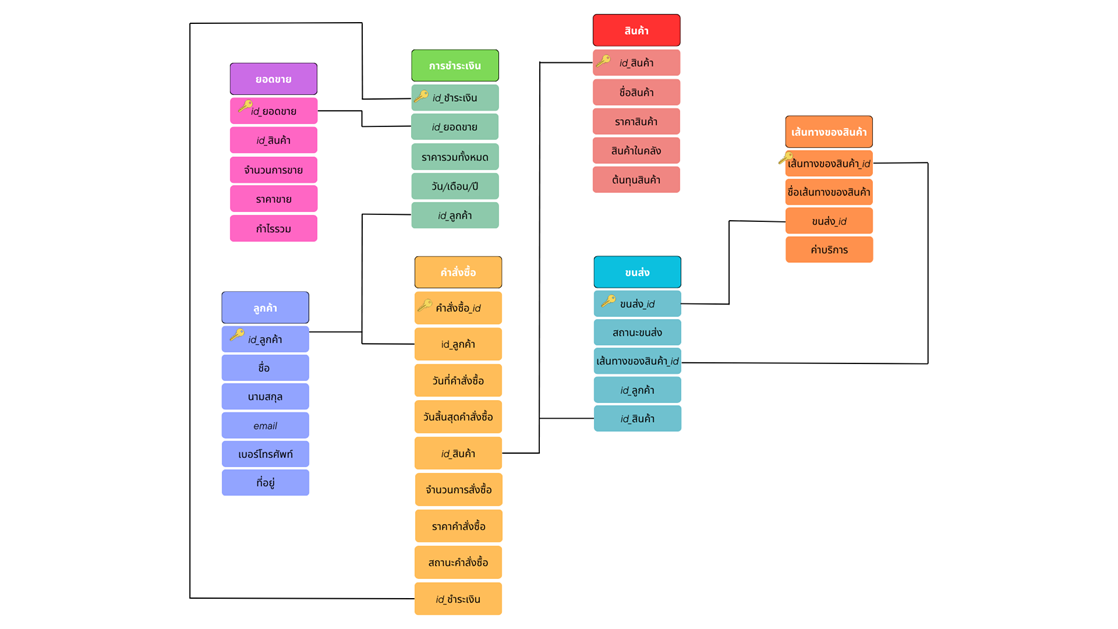
\includegraphics[width=1.5\textwidth]{er.jpg}
    \caption{ER Diagram}
\end{figure}
\chapter{SQL}
SQL เป็นภาษาโปรแกรมสำหรับจัดเก็บและประมวลผลข้อมูลในฐานข้อมูลแบบเชิงสัมพันธ์ ฐานข้อมูลแบบเชิงสัมพันธ์เก็บข้อมูลในรูปแบบตารางที่มีแถวและคอลัมน์ที่เป็นตัวแทนของหมวดข้อมูลที่แตกต่างกันและความสัมพันธ์ต่างๆ ระหว่างค่าข้อมูล สามารถใช้คำสั่ง SQL ในการจัดเก็บ ปรับปรุง ลบ ค้นหา และดึงข้อมูลจากฐานข้อมูล นอกจากนี้ยังสามารถใช้ SQL ในการรักษาและเพิ่มประสิทธิภาพการทำงานของฐานข้อมูล\\
ตัวอย่างในการสร้าง SQL ที่ใช้ในการสร้างฐานข้อมูลบริษัทผลิตน้ำเปล่า ในที่นี้จะใช้เป็นตารางของลูกค้ามายกตัวอย่าง\\
\begin{verbatim}
CREATE TABLE Customers (
    Customer_id INT PRIMARY KEY,
    Firstname TEXT,
    Lastname TEXT,
    Email TEXT,
    Phone_number NUMERIC,
    Address TEXT
);
\end{verbatim}\\
\newpage{และตัวอย่างในการใส่ข้อมูลลงในตาราง จากตัวอย่างด้านบน\\
\begin{verbatim}
INSERT INTO users (Customer_id, Firstname, Lastname, Email, Phone_number, Address) VALUES
(1, 'Somchai', 'Sukjai', 'somchai@example.com', '812345678', 'Bangkok, Thailand'),
(2, 'Sompong', 'Dee', 'sompong@example.com', '823456789', 'Chiang Mai, Thailand'),
(3, 'Malee', 'Sri', 'malee@example.com', '834567890', 'Phuket, Thailand'),
-- ... (ข้อมูลที่เหลือ 4-30)
(30, 'Chalerm', 'Fon', 'chalerm@example.com', '801234569', 'Trat, Thailand');
\end{verbatim}}
\section{SQL ที่ใช้ในการแก้ปัญหา}
\textbf{1.ลูกค้าจะสั่งสินค้าในช่วงเดือนไหนมากที่สุด}\\
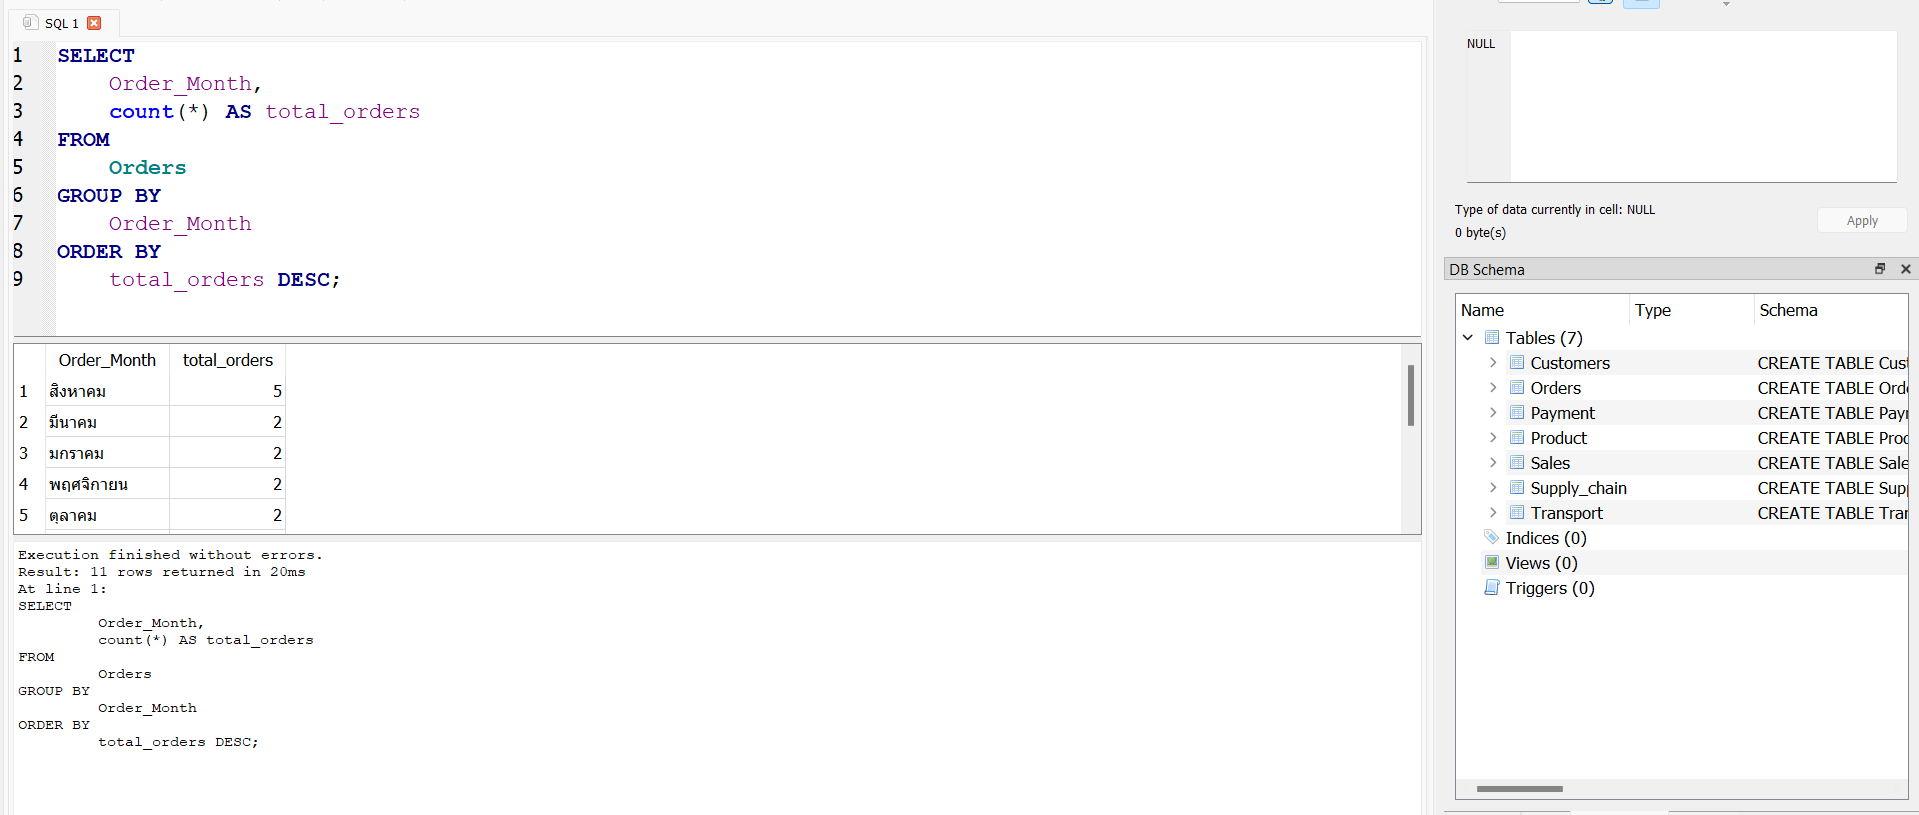
\includegraphics[width=\textwidth]{pb1.jpg}\\
\textbf{2.กำไรที่ได้แต่ละเดือนมีแนวโน้มเพิ่มขึ้นหรือลดลง}\\
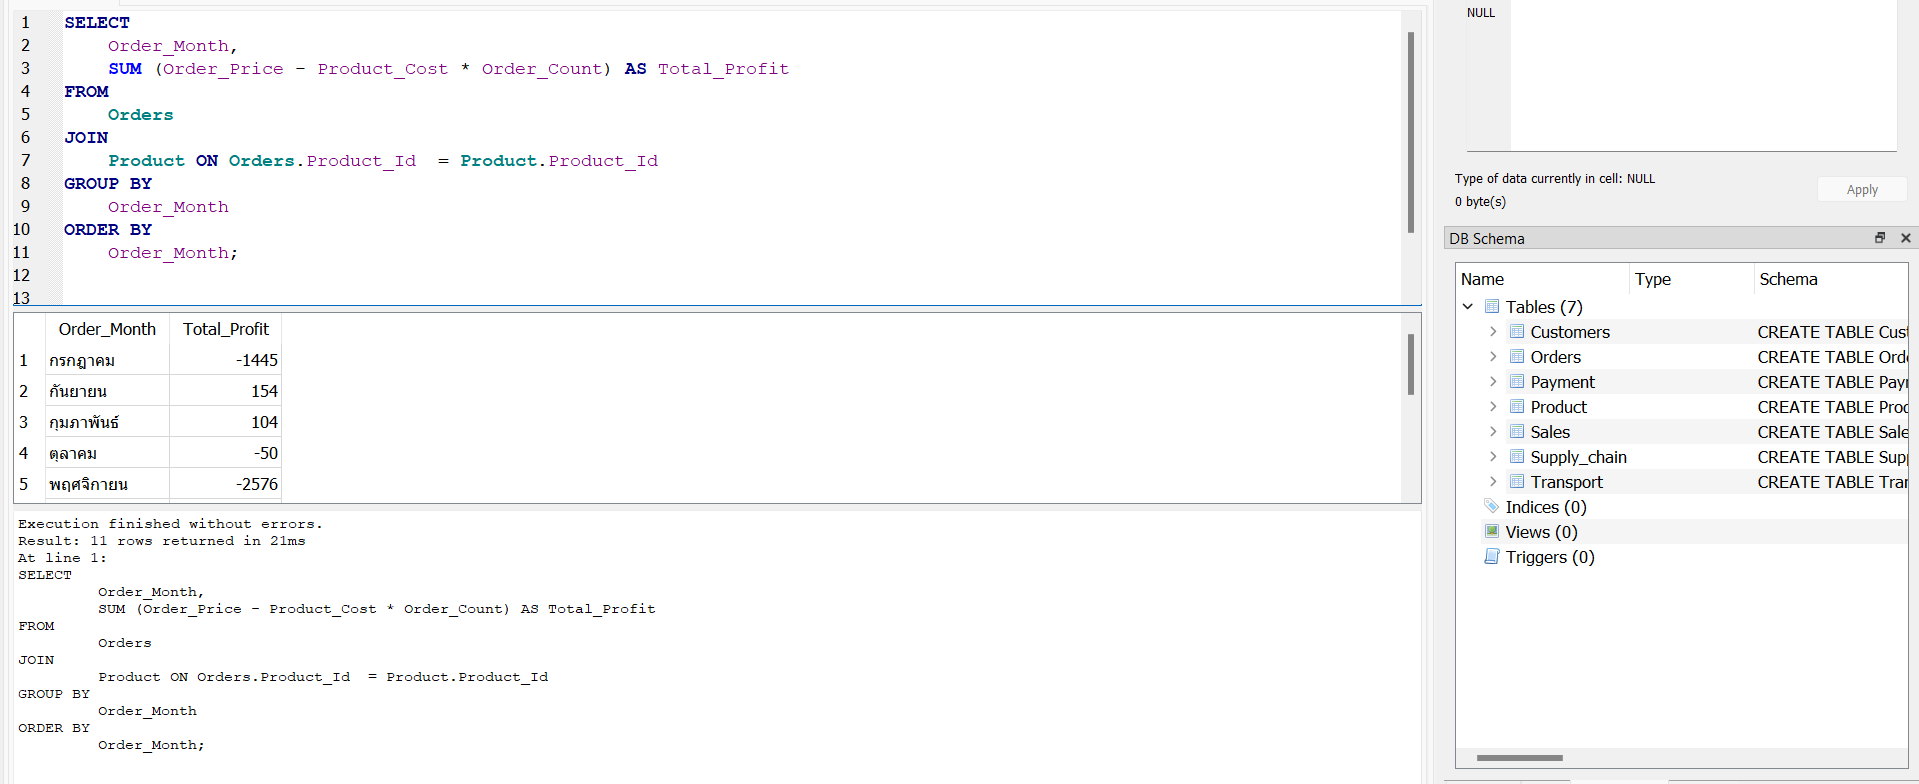
\includegraphics[width=\textwidth]{pb2.jpg}\\
\newpage{\textbf{3.การขนส่งเดือนไหนที่ค่าบริการมากที่สุด}}\\
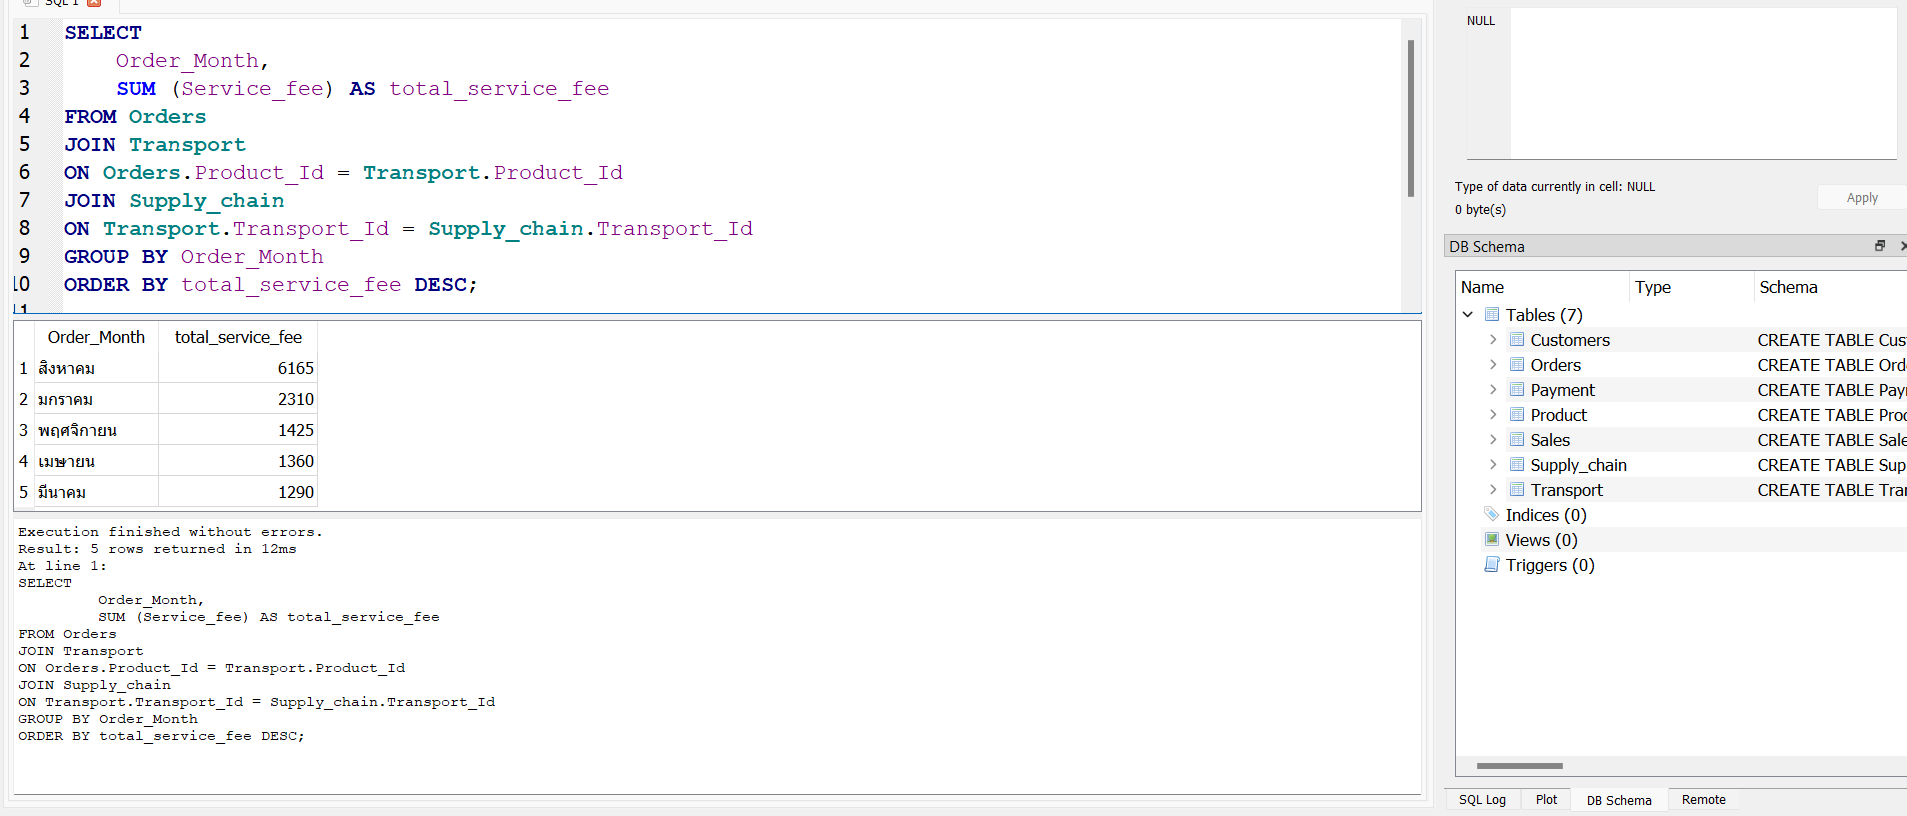
\includegraphics[width=\textwidth]{pb3.jpg}\\
\textbf{4.ลูกค้าคนไหนที่สั่งซื้อมากที่สุดในแต่ละเดือน}\\
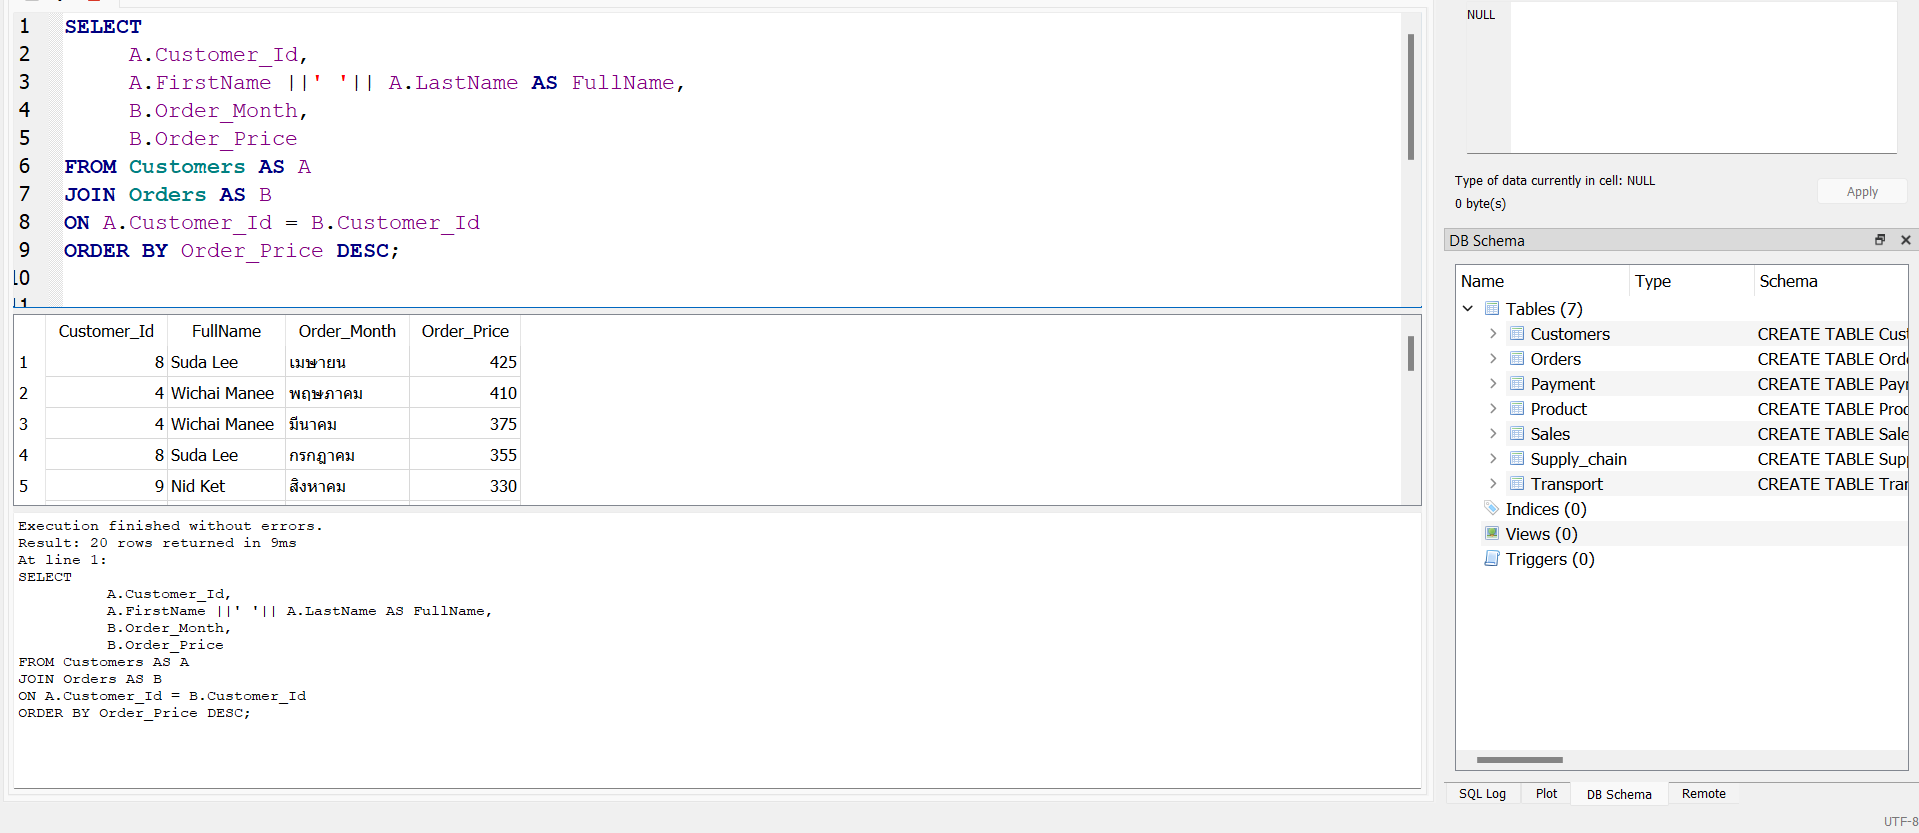
\includegraphics[width=\textwidth]{pb4.jpg}\\
\chapter{Data On Website}
การนำฐานข้อมูลขึ้นบนเว็บไซต์ คือ กระบวณการเชื่อมต่อฐานข้อมูลที่มีอยู่ภายในเครื่อง, เซิร์ฟเวอร์ หรือ ที่จัดเก็บข้อมูลภายนอก เช่น แฟลชไดร์ฟ และนำเสนอในรูปแบบเว็บไซต์ ทำให้ผู้ใช้งานสามารถเข้าถึงข้อมูลนั้นได้ผ่านอินเทอร์เน็ต\\
โดยการสร้างฐานข้อมูล เราใช้ SQLite ในการทำ เนื่องจากฐานข้อมูลนี้อยู่ในรูปแบบตารางและ ใช้ Java Script ในการพัฒนาเว็บไซต์
\section{Code ในการนำขึ้นเว็บไซต์}
\subsection{server.js}
\textbf{ส่วนแรกคือ server.js ที่เป็นการนำตารางขึ้นบนเว็บไซต์ ส่วนของการสร้างและแสดงตาราง ตัวอย่าง}
\begin{verbatim}
const express = require('express');
const bodyParser = require('body-parser');
const sqlite3 = require('sqlite3').verbose();
const path = require('path');

const app = express();
const port = 3000;

app.use(bodyParser.json());
app.use(bodyParser.urlencoded({ extended: true }));
app.use(express.static(path.join(__dirname)));

app.listen(port, () => {
    console.log(`Server running on http://localhost:${port}`)
});

const db = new sqlite3.Database('./ฐานข้อมูลบริษัทน้ำเปล่า.db');

let query = `CREATE TABLE IF NOT EXISTS Product (
    Product_Id INTEGER PRIMARY KEY AUTOINCREMENT,
    Product_name TEXT,
    Product_Price NUMERIC,
    Stock NUMERIC,
    Product_cost NUMERIC
)`;

db.run(query);

app.get('/product', (req, res) => {

    let query = 'SELECT * FROM Product';

    db.all(query, (err, rows) => {
        if (err) {
            let msg = {error: err.message};
            status(500).json(msg);
        }
        res.json(rows);
    });
});
\end{verbatim}
\textbf{อีกส่วนคือ การหาข้อมูลภายในตาราง ตัวอย่าง}
\begin{verbatim}
app.get('/search-product', (req, res) => {
    const conditions = [];
    const params = [];
    if (req.query.Product_Id) {
        conditions.push('Product_Id = ?');
        params.push(req.query.Product_Id);
    }
    if (req.query.Product_name) {
        conditions.push('Product_name LIKE ?');
        params.push(`%${req.query.Product_name}%`);
    }
    if (req.query.Product_Price) {
        conditions.push('Product_Price = ?');
        params.push(req.query.Product_Price);
    }
    if (req.query.Stock) {
        conditions.push('Stock = ?');
        params.push(req.query.Stock);
    }
    if (req.query.Product_cost) {
        conditions.push('Product_cost = ?');
        params.push(req.query.Product_cost);
    }
    let query = 'SELECT * FROM Product';
    if (conditions.length > 0) {
        query += ' WHERE ' + conditions.join(' AND ');
    }
    db.all(query, params, (err, rows) => {
        if (err) {
            return res.status(500).json({ error: err.message });
        }
        res.json(rows);
    });
});
\end{verbatim}
\subsection{HTML}
\textbf{ส่วนที่สองคือ HTML หรือส่วนที่แสดงบนเว็บไซต์ ตัวอย่าง}
\begin{verbatim}
<!DOCTYPE html>
<html lang="en">
<head>
    <meta charset="UTF-8">
    <meta name="viewport" content="width=device-width, initial-scale=1.0">
    <title>บริษัทน้ำเปล่า</title>
    <link href="style1.css" rel="stylesheet" type="text/css">
</head>
<head>
    <meta charset="UTF-8">
    <meta name="viewport" content="width=device-width, initial-scale=1.0">
    <title>Water Company Database</title>
    <link rel="stylesheet" href="style1.css">
</head>
<body>
    <div class="container">
        <img src="Logo.png" alt="WATER WATER Logo" class="logo">
        <h1>ฐานข้อมูลบริษัทน้ำเปล่า</h1>
        <nav>
            <a href="home.html">Home</a>
            <a href="about.html">About</a>
            <a href="product.html">Product</a>
            <a href="order.html">Order</a>
            <a href="payment.html">Payment</a>
            <a href="contact.html">Contact</a>
        </nav>
        <div class="content">
            <p>ยินดีต้อนรับสู่ฐานข้อมูลของบริษัทน้ำเปล่า</p>
            <p>เลือกหมวดหมู่เพื่อดูข้อมูล</p>
        </div>
    </div>
</body>
<body>
    <h1>Product</h1>
        <form id="productForm">
            <input type="number" id="Product_Id" placeholder="Product_Id">
            <input type="text" id="Product_name" placeholder="Product_name">
            <input type="number" id="Product_Price" placeholder="Product_Price">
            <input type="number" id="Stock" placeholder="Stock">
            <input type="number" id="Product_cost" placeholder="Product_cost">
            <button type="submit">Find Product</button>
        </form>
    <table id="productList">
        <tr>
            <th>Product_Id</th>
            <th>Product_name</th>
            <th>Product_Price</th>
            <th>Stock</th>
            <th>Product_cost</th>
        </tr>
    </table>
    <br>
    <h1>Orders</h1>
        <form id="ordersForm">
            <input type="number" id="Order_Id" placeholder="Order_Id">
            <input type="number" id="Order_Customer_Id" placeholder="Customer_Id">
            <input type="number" id="Order_Payment_Id" placeholder="Payment_Id">
            <input type="text" id="Order_Date" placeholder="Order_Date">
            <input type="text" id="Order_Status" placeholder="Order_Status">
            <button type="submit">Find Order</button>
        </form>
    <table id="ordersList">
        <tr>
            <th>Order_Id</th>
            <th>Customer_Id</th>
            <th>Payment_Id</th>
            <th>Order_Date</th>
            <th>Order_Deadline</th>
            <th>Order_Month</th>
            <th>Order_Year</th>
            <th>Product_Id</th>
            <th>Order_Count</th>
            <th>Order_Price</th>
            <th>Order_Status</th>
        </tr>
    </table>
\end{verbatim}
\textbf{ส่วนที่แสดงบนหน้าเว็บไซต์นี้ นอกจากส่วนของฐานข้อมูลแล้วยังมีส่วนอื่นๆ เช่น หน้าหลัก, เกี่ยวกับ หรือ ช่องทางการติดต่อ เช่น}
\begin{verbatim}
//Home หรือ หน้าหลัก
<!DOCTYPE html>
<html lang="en">
<head>
    <meta charset="UTF-8">
    <title>บริษัทน้ำเปล่า</title>
    <meta name="viewport" content="width=device-width, initial-scale=1.0">
    <link href="style.css" rel="stylesheet" type="text/css">
</head>
<body>
    <div class="container">
        <img src="Logo.png" alt="WATER WATER Logo" class="logo">
        <h1>WATER WATER</h1>
        <nav>
            <a href="about.html">About</a>
            <a href="product.html">Product</a>
            <a href="payment.html">Payment</a>
            <a href="order.html">Order</a>
            <a href="contact.html">Contact</a>
            <a href="table.html">Database</a>
        </nav>
        <div class="content">
            <h2>ยินดีต้อนรับ</h2>
            <p>เลือกหมวดหมู่จากเมนูเพื่อดูข้อมูลเพิ่มเติม</p>
            <h2>สินค้าแนะนำ</h2>
            <div class="recommended-products">
                <div class="product">
                    <img src="product.png" alt="น้ำดื่ม 500 มล." class="product-image">
                    <h3>น้ำดื่ม 500 มิลลิลิตร</h3>
                    <p>ราคา: 10 บาท</p>
                    <p>น้ำดื่มคุณภาพสูงในขวด PET ขนาดพกพา</p>
                </div>
                <div class="product">
                    <img src="product1.png" alt="น้ำดื่ม 1 ลิตร" class="product-image">
                    <h3>น้ำดื่ม 1 ลิตร</h3>
                    <p>ราคา: 15 บาท</p>
                    <p>น้ำดื่มบริสุทธิ์เหมาะสำหรับการบริโภคในบ้านหรือองค์กร</p>
                </div>
                <div class="product">
                    <img src="product2.png" alt="น้ำดื่ม 1.5 ลิตร" class="product-image">
                    <h3>น้ำดื่ม 1.5 ลิตร</h3>
                    <p>ราคา: 20 บาท</p>
                    <p>น้ำดื่มขนาดใหญ่สำหรับการเดินทางหรือกิจกรรมกลางแจ้ง</p>
                </div>
            </div>
            <div class="info-box">
                <h2>พันธกิจของเรา</h2>
                <p>เรามุ่งมั่นที่จะเป็นผู้นำด้านผลิตภัณฑ์น้ำดื่มที่ใส่ใจสิ่งแวดล้อม ด้วยการใช้บรรจุภัณฑ์ที่สามารถรีไซเคิลได้ รวมถึงสนับสนุนการอนุรักษ์น้ำและทรัพยากรธรรมชาติ</p>
                <h2>สินค้าของเรา</h2>
                <p>บริษัทเรามีสินค้าน้ำดื่มหลายรูปแบบ เช่น น้ำดื่มขวด PET ขนาด 500 มิลลิลิตร, 1 ลิตร, และ 1.5 ลิตร เพื่อตอบสนองความต้องการของลูกค้าในทุกโอกาส ทั้งเพื่อการบริโภคส่วนตัวและการใช้งานในองค์กร</p>
                <h2>มาตรฐานและคุณภาพ</h2>
                <p>เราใช้เทคโนโลยีการกรองและฆ่าเชื้อที่ทันสมัย เพื่อให้มั่นใจได้ว่าผลิตภัณฑ์น้ำดื่มของเรามีคุณภาพที่ปลอดภัยต่อสุขภาพ ทุกขวดของน้ำดื่มผ่านการตรวจสอบโดยผู้เชี่ยวชาญก่อนถึงมือผู้บริโภค</p>
                <h2>การดูแลลูกค้า</h2>
                <p>เรามีศูนย์บริการลูกค้าที่พร้อมให้บริการทุกวัน ตั้งแต่เวลา 8.00 น. ถึง 17.00 น. โดยทีมงานของเราพร้อมให้คำแนะนำเกี่ยวกับผลิตภัณฑ์ และตอบคำถามที่เกี่ยวข้องกับการสั่งซื้อและการชำระเงิน</p>
                <h2>ร่วมเป็นส่วนหนึ่งในการอนุรักษ์สิ่งแวดล้อม</h2>
                <p>เราสนับสนุนให้ลูกค้าร่วมกันลดการใช้ขวดพลาสติกแบบใช้ครั้งเดียว และหันมาใช้บรรจุภัณฑ์ที่สามารถรีไซเคิลหรือใช้ซ้ำได้ เพื่อช่วยลดปริมาณขยะพลาสติกในธรรมชาติ</p>
            </div>
        </div>
    </div>
</body>
</html>
//About หรือ เกี่ยวข้องกับเรา
<!DOCTYPE html>
<html lang="en">
<head>
    <meta charset="UTF-8">
    <meta name="viewport" content="width=device-width, initial-scale=1.0">
    <title>เกี่ยวกับเรา - บริษัทน้ำเปล่า</title>
    <link href="style.css" rel="stylesheet">
</head>
<body>
    <div class="container">
        <img src="Logo.png" alt="WATER WATER Logo" class="logo">
        <nav>
            <a href="home.html">Home</a>
            <a href="product.html">Product</a>
            <a href="order.html">Order</a>
            <a href="payment.html">Payment</a>
            <a href="contact.html">Contact</a>
            <a href="table.html">Database</a>
        </nav>
    <div class="info-box">
        <h2>เกี่ยวกับเรา</h2>
            <p>บริษัทน้ำเปล่ามีความมุ่งมั่นในการส่งมอบน้ำดื่มบริสุทธิ์ที่ดีที่สุดให้กับลูกค้า ด้วยเทคโนโลยีที่ทันสมัยและกระบวนการผลิตที่ได้มาตรฐาน</p>
            <h2>ประวัติของบริษัท</h2>
            <p>ก่อตั้งขึ้นในปี 2567 บริษัทน้ำเปล่ามุ่งมั่นที่จะผลิตน้ำดื่มคุณภาพสูง เพื่อสนับสนุนความต้องการของลูกค้าในทุกกลุ่มเป้าหมาย ด้วยการใช้วัตถุดิบที่ดีที่สุดและการผลิตที่ปลอดภัย</p>
            <h2>วิสัยทัศน์</h2>
            <p>เรามีวิสัยทัศน์ในการเป็นผู้นำด้านการผลิตน้ำดื่มที่มีคุณภาพสูงและใส่ใจต่อสิ่งแวดล้อม โดยเรามีการลงทุนในเทคโนโลยีที่เป็นมิตรต่อสิ่งแวดล้อม และใช้บรรจุภัณฑ์ที่สามารถรีไซเคิลได้</p>
            <h2>ทีมงานของเรา</h2>
            <p>เรามีทีมงานที่มีความเชี่ยวชาญและประสบการณ์ในการผลิตน้ำดื่มอย่างมืออาชีพ ที่พร้อมให้บริการและแนะนำผลิตภัณฑ์น้ำดื่มที่เหมาะสมกับความต้องการของลูกค้า</p>
            <img src="water1.png" class="image-frame">
    </div>
    </div>
</body>
</html>
//Contact หรือ ช่องทางการติดต่อ
<!DOCTYPE html>
<html lang="en">
<head>
    <meta charset="UTF-8">
    <meta name="viewport" content="width=device-width, initial-scale=1.0">
    <title>ติดต่อเรา - บริษัทน้ำเปล่า</title>
    <link href="style.css" rel="stylesheet">
</head>
<body>
    <div class="container">
        <img src="Logo.png" alt="WATER WATER Logo" class="logo">
        <nav>
            <a href="home.html">Home</a>
            <a href="about.html">About</a>
            <a href="product.html">Product</a>
            <a href="order.html">Order</a>
            <a href="payment.html">Payment</a>
            <a href="table.html">Database</a>
        </nav>
        <div class="content">
            <h1>ติดต่อเรา</h1>
            <p>ที่อยู่: 123 ตำบลคลองหก อำเภอคลองหลวง จังหวัดปทุมธานี</p>
            <p>เบอร์ติดต่อ: 02-123-4567</p>
            <p>อีเมล: waterwater@watercompany.com</p>
            <img src="face.png" alt="WATER WATER Logo" class="logo">
            <p>Facebook: WATER WATER</p>
            <img src="line.png" alt="WATER WATER Logo" class="logo">
            <p>Line: @WATER WATER</p>
            <img src="ig.png" alt="WATER WATER Logo" class="logo">
            <p>Instagran: WATER_WATER</p>
        </div>
    </div>
</body>
</html>
\end{verbatim}
\subsection{script.js}
\textbf{ส่วนที่สามคือ script.js ตัวอย่าง}
\begin{verbatim}
async function fetchProducts() {
    const response = await fetch('/product');
    const products = await response.json();
    displayProducts(products);
}

function displayProducts(products) {
    const productList = document.getElementById('productList');
    productList.innerHTML = `
<tr>
<th>Product_Id</th>
<th>Product_name</th>
<th>Product_Price</th>
<th>Stock</th>
<th>Product_cost</th>
</tr>`;
 
    products.forEach(product => {
        productList.innerHTML += `
<tr>
<td>${product.Product_Id}</td>
<td>${product.Product_name}</td>
<td>${product.Product_Price}</td>
<td>${product.Stock}</td>
<td>${product.Product_cost}</td>
</tr>`;
    });
}
// Search event listeners
document.getElementById('productForm').addEventListener('submit', async (e) => {
    e.preventDefault();
    const searchParams = {
        Product_Id: document.getElementById('Product_Id').value,
        Product_name: document.getElementById('Product_name').value,
        Product_Price: document.getElementById('Product_Price').value,
        Stock: document.getElementById('Stock').value,
        Product_cost: document.getElementById('Product_cost').value
    };
    const response = await fetch('/search-product?' + new URLSearchParams(
        Object.entries(searchParams).filter(([_, value]) => value !== '')
    ));
    const products = await response.json();
    displayProducts(products);
});
fetchProducts();
\end{verbatim}
\chapter{Data On GIT}

\end{document}